% Copy-pasted from original. Maybe in an appendix?
\section{Pruebas de consistencia}
Antes de obtener resultados, es importante verificar la calidad y
correctitud del código empleado. Para ello, se efectuaron diversas
simulaciones en las que el resultado fuera conocido de antemano.

\begin{description}
  \item[Modelo de Ising]
  Como puede verse en la figura \ref{fig:ising}, la temperatura crítica
  es consistente con el valor de la literatura\cite{isingtemp},
  $T\sub{C}≃4.52$.

  \item[Ecuaciones de Schwinger-Dyson]

  Para validar la correcta distribución estadística de los espines en
  las simulaciones se empleó un set de las ecuaciones de
  Schwinger-Dyson\cite{schwinger}. Para cualquier $β$,
  \begin{equation}
    \frac{1}{V}\sum_{i} e^{-2β\Ham_i} ≃ 1
  \end{equation}

  donde $\Ham_i = - \sum_{j} σ_iσ_j$ es el término del hamiltoniano $\Ham =
  \sum_{} \Ham_i$ correspondiente al espín $σ_i$, con $σ_j$ los primeros
  vecinos de $σ_i$.

  El observable se puede promediar sobre los $L^3$ espines de la red
  para obtener más estadística, pero es inutil tratar de emplear la
  desviación estandar para acotar su valor, ya que ésta es enorme
  (del orden de 10) debido a las fuertes fluctuaciones de
  la exponencial. En lugar de ello, se realizó un \textit{bootstrap}
  (apéndice \ref{chap:bootstrap}).

  En la figura \ref{fig:SD} pueden verse los resultados, compatibles con
  lo esperado (media $1$).
  \item[Energía]
    \begin{figure}
      \centering
      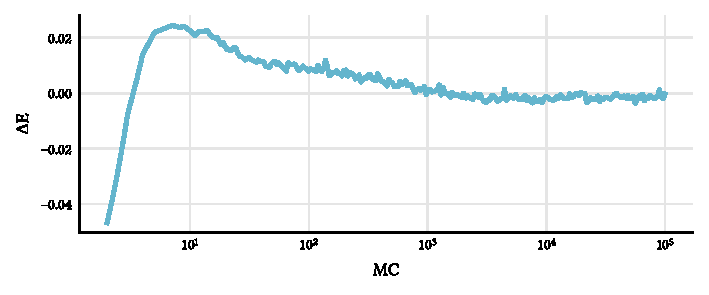
\includegraphics{../study_cases/sergio_energy/comparison_mini.pdf}
      \caption{El valor de la energía converge al mismo valor
        independientemente del autor del software. Notar que la
        energía converge antes hacia el valor de equilibrio para los
        datos propios, debido a que la \textit{Janus Collaboration}
        emplea un algoritmo de \textit{Heat Bath}.}
      \label{fig:energyvssergio}
    \end{figure}
    Se comparó el valor de la energía para un quench directo a
    diferentes temperaturas con datos obtenidos por la \textit{Janus
      collaboration} en un ordenador dedicado, con un software completamente
    distinto. Como puede verse en la figura \ref{fig:energyvssergio},
    ambos programas dan resultados compatibles para $E(MC→∞)$.

  \item[Correlación]
  Por último, se trató de ver si la correlación entre espines a
  distintos tiempos seguía, tal y como propone la
  literatura\cite{corrparisi}, la forma funcional
  \begin{equation}
    C(t_w,t_w + t_0) = a(t_0) + b(t_0) t_w ^{-c(t_0)}
  \end{equation}
  El ajuste a la función propuesta es bueno bajo inspección visual
  para el régimen de $t_w$ elevado, condiciones empleadas en la
  deducción de la fórmula en el artículo consultado.
\end{description}



\begin{figure}
  \centering
  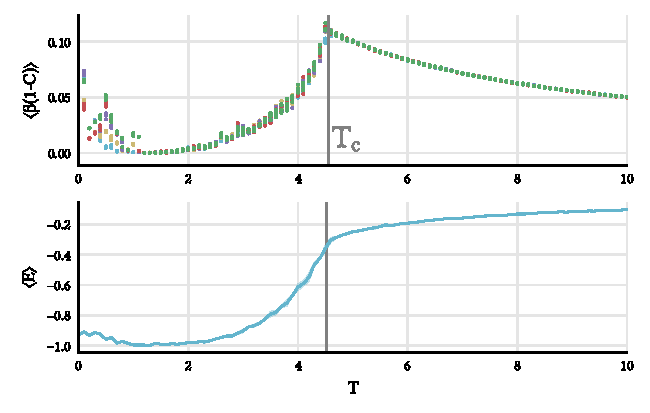
\includegraphics{../study_cases/ising/corrplot.pdf}
  \caption{La temperatura crítica obtenida para el modelo de Ising
    (cúspide de la susceptibilidad, $T\sub{C} ∼4.5$) es
    consistente con la de la literatura (marcada con una línea
    vertical). Se emplearon $5$ valores equiespaciados de $t_0 ∈
    [10,10^3]$, $L=16$ y $10^3$ iteraciones de termalización.}
  \label{fig:ising}
\end{figure}

\begin{figure}
  \centering
  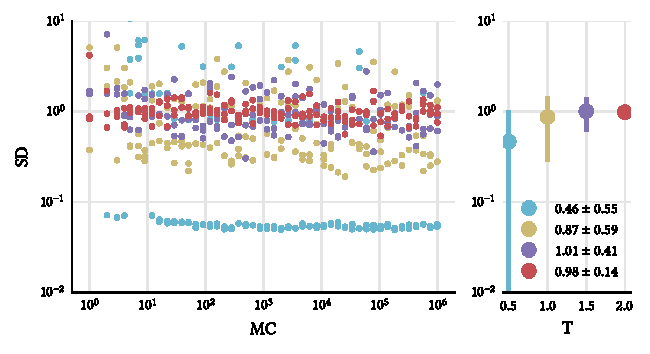
\includegraphics{../study_cases/schwinger/SD.pdf}
  \caption{A pesar de la enorme variabilidad del observable, el
    resultado de la ecuación de Schwinger-Dyson posee una media
    compatible con el valor esperado, $1$. Se muestran las mediciones
    individuales del observable promediadas sobre espines para cada
    temperatura en la figura izquierda, y un bootstrap de la media con
    cobertura de un σ para cada temperatura empleada a la derecha.}
  \label{fig:SD}
\end{figure}

\begin{figure*}
  \centering
  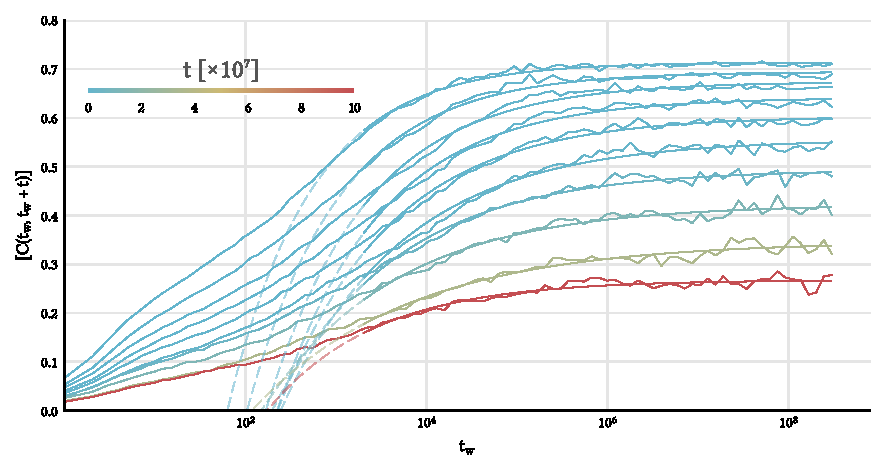
\includegraphics{../study_cases/correlation/fit.pdf}
  \caption{El ajuste de $C(t_w,t_w+t_0)$ a una ley potencial del tipo
    $a+bt_w^{-c}$ es aceptable para $t_w$ alta.}
  \label{fig:SD}
\end{figure*}
